\chapter{Phase 1 - Keine Veränderungen an den APs}
\label{ch:phase1}
In einem ersten Schritt sollten laut Aufgabenstellung keine Veränderungen an den Access Points vorgenommen werden können.
Weil die Ortung deshalb auf WLAN basieren muss sind die Knoten im Folgenden immer APs. 
Ein Tag ist eine mobile Einheit, umgekehrt gilt dies jedoch nicht, da auch alle anderen WLAN-fähigen Geräte, wie Smartphones und Laptops, eine mobile Einheit sein kommen. \\
Die Unveränderlichkeit bedeutet insbesondere auch, dass keine Messwerte verwendet werden können, die direkt am AP gemessen werden müssen und nicht als Teil der 802.11 in das dahinterliegende Netzwerk weitergeleitet werden.
Da time of arrival Synchronisation und präzise Timer bei den APs vorraussetzt und time difference of arrival nur von den APs gemessen werden kann, eignen sich diese Messgrößen nicht für diese Aufgabenstellung.
Received signal strength und roundtrip time of flight können auf der mobilen Einheit gemessen werden, nicht jedoch an den APs, da die in der PHY- beziehungsweise MAC-Schicht gemessenen Werte nicht an weitere Empfänger im Netzwerk propagiert werden. 
Somit scheidet die direkte Fernlokalisierung mangels Messgrößen aus, es wird stattdessen eine indirekte Fernlokalisierung durchgeführt bei der die mobile Einheit eine Selbstlokalisierung durchführt und das Ergebnis dem Ortungsserver über eine Datenverbindung mitteilt.


\section{Vorherige Arbeiten}
\label{ch:phase1:sec:vorherige}
Zunächst werden vorherige Arbeiten behandelt, es werden sowohl wissenschaftliche als auch kommerzielle Lösungen betrachtet.


\subsection{WiFi-LLS}
\label{ch:Vorherige:sec:LLS}
Chen et al. stellen mit dem WiFi-based Local Location System (WiFi-LLS) ein System zur indirekten Fernlokalisierung vor \cite{chen2007design}.
Als Messgröße wird die Stärke des empfangenen Signals (received signal strength, RSS) genutzt, diese wird laut 802.11 Spezifikation als Index (RSSI) von der Hardware zurückgegeben. \\
Für die Ortung wird zunächst der RSSI von Paketen naher APs gemessen und zusammen mit der MAC-Adresse der mobilen Einheit in ein Paket gepackt und an den Ortungsserver versendet.
Anschließend wird auf dem Ortungsserver ein theoretisches Signalausbreitungsmodell $P(d) = P(d_0) - 10log_{10}(\frac{d}{d_0})^n - OAF$ mit der Distanz $d$, der Signalstärke $P(d)$ und der Referenzdistanz $d_0 = 1m$ zur Bestimmung der Position der mobilen Einheit verwendet. \\
$P(d_0)$, der Pfadverlustexponent $n$ und der Hindernisdämpfungsfaktor $OAF$ müssen bestimmt werden, jedoch lassen sich $P(d_0)$ und $n$ auf einer einzelnen Teststrecke mit unterschiedlichen Abständen von AP und mobiler Einheit bestimmen. $OAF$ kann sogar für einen Gebäudetyp einmalig bestimmt werden.
Dadurch hat das Modell einen konstanten Aufwand. 
Dies ist für Baustellen interessant, da sich diese Werte einmalig messen und dann sogar über mehrere gleichartige Baustellen übertragen ließen.\\
In dieser Veröffentlichung steht die Ortungsgenauigkeit im Vordergrund und es werden keine Angaben zum Energieverbrauch gemacht. 
Als Referenz kann dienen, dass die mobile Einheit bei WiFi-LLS alle 5 Sekunden einen Scan (siehe Abschnitt \ref{ch:phase1:sec:scan}) durchführt, dann werden die Signalstärken entdeckten APs zusammen mit der eigenen MAC-Adresse in XML codiert und das so erzeugte Paket an den Ortungsserver versendet.

\subsection{AiRISTA Flow RTLS}
Ekahau bietet unter der Marke \textit{AiRISTA Flow RTLS} eine, zu WiFi-LLS ähnliche, Lösung kommerziell an \cite{airista2017airista}.
Ihr Ekahau B4 Badge Tag ermittelt regelmäßig den RSSI zu nahegelegenen Access Points und versendet diese an einen Ortungsserver \cite{liu2007survey}.
Das Tag bietet darüber hinaus noch einige Zusatzfunktionen, so können über die Datenverbindung auch Nachrichten und Alarmierungen an das Tag gesendet werden und die drei angebrachten Knöpfe können programmiert werden.\\
Bezüglich des Energieverbrauchs gibt sich das Informationsblatt des B4 Badge Tag vage: Das Tag soll abhängig vom Ortungsintervall wochenlang halten, danach muss der $600\ mA/h$ Akku geladen werden \cite{ekahau2017b4}.
Das Informationsblatt zum Ekahau W4, welches statt um den Hals am Handgelenk getragen wird, gibt an, dass der verbaute $530\ mA/h$ Akku bei einem Ortungsintervall von 15 Sekunden 500 Stunden (ca. 21 Tage) hält \cite{ekahau2017w4}.\\
AiRISTA Flow spricht auf ihrer Website zum Beispiel Krankenhäuser, Schulen und Regierungseinrichtungen an, hier sollen zusätzlich bewegliche Objekte, wie etwa Krankenhausbetten, geortet werden.
Die dazu verwendeten Asset Tags werden über einen Beschleunigungssensor aktiviert und können, wenn die Objekte selten bewegt werden, deutlich längere Laufzeiten erreichen \cite{ekahau2017a4}. \\

\subsection{AeroScout}
Auch das AeroScout System von Stanley Healthcare richtet sich an den medizinischen Sektor und soll Objekte und Personen orten \cite{aeroscout2017asset}, \cite{aeroscout2017staff}.
Da sich auch dieses System in das bestehende WLAN-Netzwerk einfügt, sollte es ebenfalls auf einer indirekten Fernlokalisierung beruhen und demnach ähnliche Eigenschaften bezüglich des Energieverbrauchs aufweisen.\\
Das Informationsblatt ihres T14 Tags für Personen gibt eine Laufzeit von bis zu drei Wochen, abhängig von Konfiguration und Typ des Tags, an \cite{aeroscout2017t14}. 
Eine Angabe zu dem verwendeten Typ, der Konfiguration oder der Kapazität des verbauten Akkus wird nicht gemacht.\\

\subsection{Selbstlokalisierung mit Szenenanalyse}
\label{ch:Vorherige:sec:RSS-basierte}
Prasithsangaree et al. stellen ein System zur Selbstlokalisierung vor \cite{prasithsangaree2002indoor}, es verwendet aber eine offline-Phase zum Sammeln von Fingerabdrücken für Positionen in einem Abstand von 1,5 beziehungsweise 3 Metern. 
In diesen Fingerabdrücken werden die gemessenen RSSI der von den APs empfangenen Pakete als Merkmale zusammen mit der Position als Label gespeichert.
In der anschließenden online-Phase werden die gemessenen RSSI mit den Fingerabdrücken verglichen und die Position als gewichtetes Mittel der Labels bestimmt. \\
Die offline-Phase ist natürlich im Sinne der Aufgabenstellung nicht sinnvoll, da für eine Tunnelbreite von 10m 4000 beziehungsweise 2000 Messungen pro Kilometer vorgenommen werden müssten.
Generell eignen sich Lösungen mit Szenenanalyse nicht gut für Baustellen, da diese nicht auf die potentiell höhere Genauigkeit angewiesen sind. 
Üblicherweise müssen dort sehr große Flächen vermessen werden und die Veränderungen durch den Baufortschritt führen dazu, dass regelmäßig neu gemessen werden muss.
Außerdem müssen bewegliche Störquellen wie Baumaschinen vorher aus dem Bereich entfernt werden, um unverfälschte Fingerabdrücke zu erhalten.
Der Aufwand ein System mit Szenenanalyse auf einer Baustelle zu betreiben ist deshalb sehr hoch und widerspricht der Forderung nach geringer Komplexität. \\
Die Arbeit zeigt aber die Volatilität der empfangenen Signalstärke auf, dies wurde 2011 von Lui et al. genauer untersucht \cite{lui2011differences}.
Lui et al. zeigen, dass die gemessene empfangene Signalstärke stark von der beteiligten Hardware abhängt und die Systeme jedes mal neu kalibriert werden müssen wenn sie auf ein neues AP-Modell portiert werden. 
Auf dem Areal sollte deshalb optimalerweise nur ein AP-Modell verwendet werden. \\
Abb. \ref{fig:luiRSSI} zeigt die gemessenen RSSI Werte für die von ihnen getesten Netzwerkkarten mit unterschiedlichen Distanzen, für einige Karten korreliert die empfangene Signalstärke nur sehr schwach mit der Distanz zwischen Knoten und mobiler Einheit.
Sie zeigen außerdem, dass einige AP-Modelle den RSSI speichern und nur bei größeren Veränderungen aktualisieren und dass die Antenne signifikanten Einfluss auf den protokollierten Wert hat.



\begin{figure}[h]
  \centering
	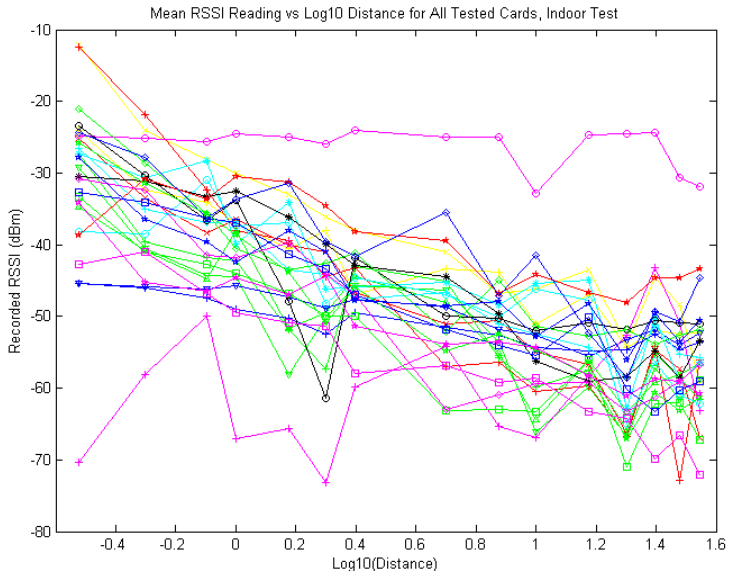
\includegraphics[width=\textwidth]{images/luiRSSI.png}
  \caption{Gemessener RSSI mit verschiedenen Access Points und Distanzen, aus \cite{lui2011differences}.}
  \label{fig:luiRSSI}
\end{figure}

\section{Grundlagen der 802.11 Spezifikation}
\label{ch:phase1:sec:grundlagen}
802.11 beschreibt eine Form der drahtlosen Datenübertragung mittels Funkwellen \cite{ieee2012macphy}.
Die Spezifikation beschreibt die physische Schicht (PHY-Layer) und den Mediumszugriff (MAC-Layer) für ein Funknetzwerk, dass sich mit den darüber liegenden Schichten des OSI-Modells in andere Netzwerke eingebunden werden kann.
Wird ein solches Netzwerk in ein Local Area Network (LAN) eingebunden spricht man üblicherweise vom Wireless Local Area Network (WLAN).
Die 1997 erstmals verabschiedete Spezifikation wurde häufig erweitert und wird in ihrer ursprünglichen Form praktisch nicht mehr angewendet, da die Datenraten zu gering sind.
Die Erweiterungen werden mit Buchstaben benannt (zum Beispiel 802.11g) und verändern entwa die verwendete Frequenz und Modulationsverfahren.\\
Zur Vermeidung von Kollisionen kommt Carrier Sense Multiple Access/Collision Avoidance (CSMA/CA) zum Einsatz.
Bei CSMA/CA wird zunächst das Medium belauscht und gewartet bis keine Signale mehr auf dem Medium sind. 
Dann muss ein Inter Frame Spacing (IFS) abgewartet werden, je nach Priorität ist dieses unterschiedlich lang (SIFS<PIFS<DIFS<EIFS), anschließend kann gesendet werden.
Tritt trotzdem eine Kollision auf, versucht der Sender es erneut mit einem längeren IFS.\\
802.11 spezifiziert ebenfalls mehrere Operationen, die beispielsweise zur Entdeckung von Ressourcen und der Authentifizierung an einer Ressource dienen, einige, für diese Arbeit wichtige Operationen werden im Folgenden beschrieben.

\subsection{Scan}
\label{ch:phase1:sec:scan}
Scan ist eine Operation zur Entdeckung von Access Points, sie kann von einer Station (Endverbraucher, zum Beispiel Smartphone oder Laptop) aktiv oder passiv ausgeführt werden \cite{ieee2012scan}.
Bei einem passiven Scan empfängt die Station und filtert die von Access Points regelmäßig gesendeten Beacons heraus, diese gelten dann als entdeckt.
Ein Beacon Frame ist ein Management Frame, der dazu gedacht ist, technische Möglichkeiten des APs zu bewerben, zum Beispiel die möglichen Datenraten und Zeitstempel zur Synchronisierung.
Versteckte APs senden keine Beacons. \\
Bei einem aktiven Scan sendet die Station einen Probe Request aus, dieser kann sowohl an alle APs (broadcast) als auch an einen speziellen AP adressiert sein.
Ein Probe Requests bewirbt, ähnlich wie ein Beacon, die technischen Möglichkeiten der Station.
Der addressierte AP, beziehungsweise im Falle des broadcasts alle APs, beantwortet den Probe Request mit einer Probe Response in der er mitteilt welche der beworbenen Funktionen er ebenfalls unterstützt, die Station schließt den Vorgang mit einem Acknowlegement ab. \\
Das 2,4GHz ISM-Band wird in Europa in 13 je 10MHz breite Kanäle aufgeteilt, da ein AP immer nur auf einem Kanal aktiv ist müsste jeder Kanal gescannt werden.
Praktisch werden jedoch breitere Kanäle verwendet, 802.11g verwendet beispielsweise 20MHz breite Kanäle, so dass effektiv nur die Kanäle 1, 5, 9 und 13 geprüft werden müssen. \\
Tabelle \ref{table:management} listet alle in der 802.11 Spezifikation gelisteten Management Frames.
Ein Management Frame wird durch die Typenbits markiert und durch die Bits für den Subtypen weiter unterschieden.

\begin{table}[h]
	\centering
	\caption{Management Frames nach 802.11 \cite{ieee2012management}}
	\label{table:management}
	\begin{tabular}{l|l|l}
		Type & Subtype & Beschreibung \\
		\hline
		00 & 0000 & Association Request  \\
		00 & 0001 & Association Response  \\
		00 & 0010 & Reassociation Request  \\
		00 & 0011 & Reassociation Response  \\
		00 & 0100 & Probe Request  \\
		00 & 0101 & Probe Response  \\
		00 & 0110 & Timing Advertisement  \\
		00 & 0111 & Reserved  \\
		00 & 1000 & Beacon  \\
		00 & 1001 & ATIM  \\
		00 & 1010 & Disassociation  \\
		00 & 1011 & Authentification  \\
		00 & 1100 & Deauthentification  \\
		00 & 1101 & Action  \\
		00 & 1110 & Action No Ack  \\
		00 & 1111 & Reserved  \\
	\end{tabular}
\end{table}

\subsection{Join}
Aus den entdeckten APs kann nun einer ausgewählt werden um seinem Netzwerk (BSS) beizutreten \cite{ieee2012join}.
Es kann zwar geschehen, dass mehrere APs eines Netzwerks entdeckt wurden, eine Statíon kann jedoch zu jedem Zeitpunkt nur mit einem AP assoziert sein. \\
Um einem Netzwerk beizutreten muss sich die Station zunächst authentifizieren, dieser Vorgang wird über einen Authentication Frame (siehe Tabelle \ref{table:management}) initiiert \cite{ieee2012auth}. 
Das weitere Vorgehen hängt vom Authentifizierungsverfahren ab, zum Beispiel kann der AP einen verschlüsselten Challenge Text an die Station senden, der mit einem aus dem Passwort erzeugten Schlüssel entschlüsselt wird und an den AP zurück gesendet werden kann. 
Ist die Antwort korrekt bestätigt der AP den Vorgang mit einem Acknowledgement und eventuell zusätzlichen Informationen für eine Stromchiffre. \\
Anschließend kann die Station mit dem AP assoziiert werden \cite{ieee2012associate}. 
Sie erhält nun eine IP und der AP gibt dem Netzwerk bekannt, dass er für die Station zuständig ist, dies geschiet  üblicherweise über das Address Resolution Protokoll (ARP). [evtl IGMP?] \\
Ist eine Station assoziert kann sie Datenverbindungen mit anderen Teilnehmern im Netzwerk aufbauen, sie könnte beispielweise das HTTP-Protokoll nutzen um eine Webseite anzufordern.

\subsection{Reassociation}
Eine Reassociation wird durchgeführt wenn die Station keine gute Verbindung mehr zu ihrem AP hat und ein AP des selben Netzwerks verfügbar ist, der eine bessere Verbindung bietet \cite{ieee2012reassociate}.
Um diesen neuen AP zu entdecken muss zunächst ein Scan durchgeführt werden. \\
Anschließend sendet die Station einen Reassociation Request an den neuen AP, im Reassociation Request wird der alte AP benannt, so dass der neue AP überprüfen kann, ob die Station tatsächlich mit ihm assoziert ist, gepufferte Pakete von ihm entgegennehmen und die Assoziation mit ihm auflösen kann.
Der Kommunikationsvorgang zwischen den APs wird auch als Handoff bezeichnet, wird dieser erfolgreich abgeschlossen antwortet der neue AP der Station mit einer Reassiciation Response.
Abschließend wird dem Netzwerk die neue Assoziation mittels ARP mitgeteilt.

\begin{figure}[h]
  \centering
	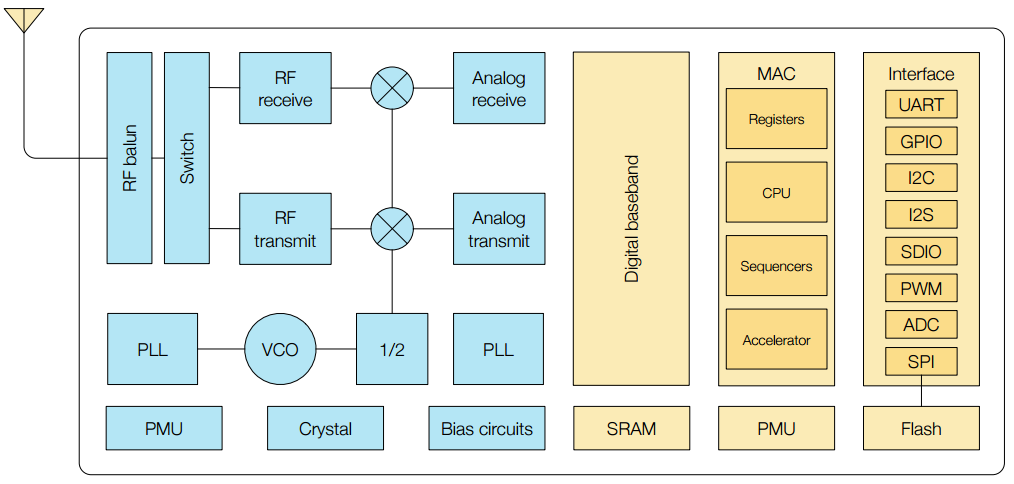
\includegraphics[width=\textwidth]{images/espblock.png}
  \caption{Blockdiagramm des ESP8266, aus \cite{espressif2017esp8266}}
  \label{fig:espblock}
\end{figure}

\section{ESP8266}
Der ESP8266 soll als Hardware für das Tag eingesetzt werden, dabei handelt es sich um einen Microcontroller von Espressif.
Der Esp8266 besitzt neben einer CPU eine 802.11b/g/n"-/e/i-fähige WLAN-Einheit und diverse andere, kabelgebundene Kommunikationsstandards wie zum Beispiel GPIO, I2C und SPI, siehe Abb. \ref{fig:espblock}. \\
Da der ESP8266 selbst weder über Flashspeicher, noch über eine Antenne verfügt wird er auf einem Modul mit diesen Komponenten verbaut, die in dieser Arbeit betrachteten Module sind das ESP12-S und das ESP12-F.
Das neuere ESP12-F sollte eine höhere Reichweite bei der Funkübertragung entfalten, dies wird noch Gegenstand eines Experiments sein.
Abb. \ref{fig:espmodules} zeigt die beiden Module nebeneinander, die unterschiedlichen Antennenformen sind deutlich zu erkennen.\\
Espressif gibt im Datenblatt auch Aufschluss über den Energieverbrauch des ESPs, siehe dazu Abb. \ref{fig:esppower}.
Für die Prototypenentwicklung wird ein ESP12-S Modul auf einem Adafruit Feather Huzzah verwendet, dieses stellt mit dem CP2104 eine serielle Schnittstelle zum ESP her, reguliert die Spannung für das Modul auf 3,3V und bringt den 2mm Pinabstand des ESP12-S Moduls auf die für Breadboards üblichen 2,5mm.
Das Adafruit Feather Huzzah mit ESP12-S ist in Abb. \ref{fig:espmodules} links abgebildet.

\begin{figure}[h]
  \centering
	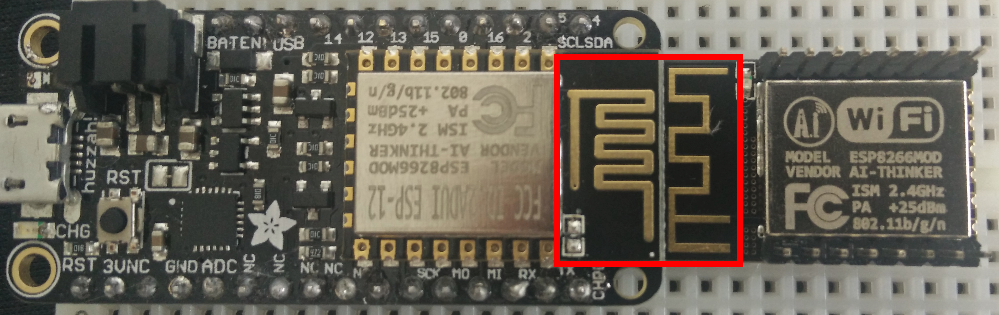
\includegraphics[width=\textwidth]{images/espmodules.png}
  \caption{Vergleich der Antennen, links: ESP12-S verbaut auf einem Adafruit Feather Huzzah, rechts: ESP12-F}
  \label{fig:espmodules}
\end{figure}

\begin{figure}[h]
  \centering
	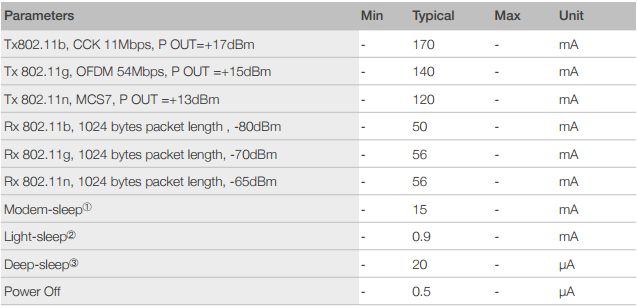
\includegraphics[width=\textwidth]{images/esppower.png}
  \caption{Energieverbrauch des ESP8266 bei verschiedenen Operationen, aus \cite{espressif2017esp8266}}
  \label{fig:esppower}
\end{figure}


\subsection{ESP8266 Arduino Core}
Eine einfache Möglichkeit den ESP8266 zu programmieren stellt die bekannte Arduino IDE dar \cite{banzi2017arduino}.\\
Unter Windows muss zunächst der Treiber für den \textit{CP2104 USB-to-Serial Chip} installiert werden, auf Linux und Mac entfällt dieser Schritt \cite{fried2017feather}.
Nach der Installation der Arduino IDE muss dort in den Einstellungen unter \textit{Additional Boards Manager URLs} die URL \url{http://arduino.esp8266.com/stable/package_esp8266com_index.json} hinzugefügt werden.  
Nach einem Neustart der IDE kann im \textit{Boards Manager} das Paket für den ESP8266 heruntergeladen werden und anschließend das Board \textit{Adafruit HUZZAH ESP8266} ausgewählt werden. \\
Ist das Board über USB mit dem Computer verbunden kann nun eigener Code oder eines der Beispiele aus \textit{Examples for Adafruit HUZZAH ESP8266} mit STRG+U auf den ESP geladen werden. 
Dieser Vorgang wird im Folgenden als flashen bezeichnet. \\
Der ESP8266 Arduino Core wird als Open Source Projekt gepflegt und setzt die ESP Open SDK auf einen, für die Arduino IDE üblichen Stil um \cite{arduino2017core}. 
Dabei wird möglichst die Kompatibilität zu Arduino gewahrt, das führt oft dazu, dass bereitgestellte Funktionen der SDK nicht in Arduino umgesetzt wurden.
Sollten die Funktionen dennoch benötigt werden können die Header-Dateien der SDK direkt importiert werden:

\begin{verbatim}
//Hier wird ein Header des ESP8266 Arduino Core importiert
#include <ESP8266WiFi.h> 

//Hier wird ein Header der ESP Open SDK importiert
extern "C" {#include "user_interface.h"} 
\end{verbatim}

Der ESP8266 Arduino Core wurde in der Version 2.3.0 verwendet.

\subsection{ESP Open SDK}
Statt mit der Arduino Core Umsetzung der ESP Open SDK kann natürlich auch direkt mit ihr programmiert werden \cite{esp2017open}. \\
Dazu muss zunächst das Github Projekt geklont werden: \texttt{git clone --recursive \url{https://github.com/pfalcon/esp-open-sdk}.git} und anschließend mit \texttt{make} kompiliert werden.
Wurde die Kompilierung erfolgreich abgeschlossen sollte die Pfadvariable (PATH) entsprechend der Meldung des make-Tools erweitert werden. \\
Die in C geschriebenen Programme können nun mit einem modifizierten GCC-Kompiler kompiliert und anschließend mit dem esptool.py zunächst in ein Image umgewandelt und dann geflasht werden. 
Das in \textit{examples} enthaltene \textit{blinky} Beispiel beinhaltet neben dem Beispielcode eine Makefile, in der diese Schritte nachvollzogen werden können, mit \texttt{make flash} wird das Beispiel kompiliert und geflasht. \\
Programme werden in regulärem C unter Zuhilfenahme der in \texttt{/sdk/include} enthaltenen Header-Dateien geschrieben, zu beachten ist nur, dass einige Funktionen der \texttt{stdlib.h} nicht verwendet werden können.
Dies betrifft vor allem direkten Speicherzugriff wie zum Beispiel \texttt{memcpy}, hier muss stattdessen \texttt{os\_memcpy} verwendet werden.
Alle betroffenen Funktionen sind in \texttt{osapi.h} beschrieben. \\
Einige frühe Experimente zeigten, dass Programme, die mit der ESP Open SDK geschrieben wurden auf dem ESP schneller starten als solche, die mit dem ESP8266 Arduino Core geschrieben wurden.
Diese Andeutung von Ineffizienzen bei der Übersetzung von Arduino Code wurde zum Anlass genommen, für die nachfolgenden Implementierungen nach der Fertigstellung des Prototypen in Arduino ebenfalls eine Implementierung in C hinzuzufügen, um ein optimales Programm zu erhalten. \\
Die ESP Open SDK wurde in der Version 2.0.0 verwendet.



\section{WiFi-LSS Implementierung}
Die mobile Einheit des WiFi-LLS Systems führt alle 5 Sekunden einen Scan aus, kodiert die Ergebnisse in XML und versendet sie an den Ortungsserver \cite{chen2007design}.
Da der Fokus dieser Arbeit auf dem Energieverbrauch liegt werden für die Referenzimplementierung eines WiFi-LLS-Tags die Kodierung in XML durch eine simple String Kodierung ersetzt und die Ergebnisse werden über UDP an den Ortungsserver übermittelt. 
Damit wird der overhead einer TCP-Verbindung vermieden.\\
Zunächst muss sich das Tag dem Netzwerk beitreten (Join) und anschließend einen Scan ausführen und ein UDP-Paket versenden.
Da die Scan-Funktion des ESP8266 Arduino Core es nicht erlaubt den RSSI zu einem AP auszulesen muss \texttt{user\_interface.h} importiert und die Scan-Funktion der SDK direkt verwendet werden.
Um den Energieverbrauch weiter zu reduzieren, soll der ESP möglichst viel Zeit in Energiesparzuständen verbringen.
Der tiefste Schlafzustand, der dennoch eine Aufrechterhaltung der WLAN-Verbindung erlaubt ist der \texttt{light\_sleep}. 
Er wird vom ESP automatisch aufgerufen, wenn er keine Aufgaben zu erledigen hat.
Er kann aber auch manuell aufgerufen werden, beides wurde getestet.\\
Einige Parameter können gewählt werden: Insbesondere die Intervallzeit bestimmt, wie oft der ESP aktiv ist und damit auch wie viel Energie er verbraucht.
Für Mitarbeiter im Tunnel kann von einer Maximalgeschwindigkeit von $30\ km/h$ ausgegangen werden, diese wird durch Schienen- oder Lastkraftfahrzeuge erreicht. 
Die maximale Reichweite des ESP12-S beziehungsweise ESP12-F Moduls ist nicht bekannt und muss noch bestimmt werden, sie wird zwischen 50 und 100 Metern angenommen.
Es wurde daher ein Intervall von 5 Sekunden gewählt, in dieser Zeit bewegt sich ein Mitarbeiter bei $30\ km/h$ ca. $42\ m$.\\
Des Weiteren kann theoretisch die Zahl der gescannten Kanäle gewählt werden, da sich die Einflussbereiche der APs in einem WLAN-Netzwerk üblicherweise überlappen ist es aber sinnvoll diese über die 4 nichtüberlappenden Kanäle zu verteilen. 
Eine Implementierung die nur einen Kanal scannt tritt deshalb nur außer Konkurenz an.\\
Tabelle \ref{table:llsconsumption} zeigt den gemessen Energieverbrauch der Implementierungen in Arduino und C, jeweils mit und ohne manuell aufgerufenen \texttt{light\_sleep} und eine Implementierung, die nur einen Channel scannt.
Für die Tests wurde das Adafruit Feather Huzzah verwendet, es wurde mit $5\ V$ aus einer USB-Powerbank mit Energie versorgt, der Verbrauch wurde mit einem dazwischen geschalteten USB-Power-Meter gemessen.\\
Die Werte wurden stationär in einer Mietwohnung in einem 5-stöckigen Wohnhaus und damit nicht unter realen Bedingungen aufgezeichnet.
Unter realen Bedingungen finden durch die Bewegung des Mitarbeiters regelmäßig Reassizationen statt, im Gegenzug liefert ein Scan in einem Tunnel weniger Ergebnisse als in einem Wohnhaus.
Ein Test unter realen Bedingungen ist im Abschnitt \ref{kommtnoch} zu finden, er beinhaltet jedoch nur noch die Implementierung in C mit manuellem \texttt{light\_sleep} und einem Scan auf allen 4 Kanälen.

\begin{table}[h]
	\centering
	\caption{Energieverbrauch WiFi-LLS-artiger Tags}
	\label{table:llsconsumption}
	\begin{tabular}{p{3cm}|p{2.2cm}|p{1.5cm}|p{2cm}|p{2cm}|p{2cm}}
		SDK & manueller \texttt{light\_sleep} & Anzahl Kanäle & Spannung in V & $\varnothing$ Verbrauch in mA & $\varnothing$ Verbrauch in mW \\
		\hline
		Arduino Core & Nein & 4 & 5 & 22 & 110 \\
		Arduino Core & Ja & 4 & 5 & 21 & 105 \\
		ESP Open SDK & Nein & 4 & 5 & 19 & 95 \\
		ESP Open SDK & Ja & 4 & 5 & 19 & 95 \\
		\hline
		ESP Open SDK & Ja & 1 & 5 & 6,5 & 32,5 \\
	\end{tabular}
\end{table}

Die Tests zeigen, dass die Programmierung mit der ESP Open SDK einen Vorteil beim Energieverbrauch hat, dieser liegt bei ca $10\%$.
Andererseits fällt auf, dass die Reduzierung der gescannten Channel eine signifikante Senkung des Energieverbrauchs nach sich zieht, die Scan-Funktion ist also der Hauptverbraucher.\\
Um die finale Laufzeit zu bestimmen muss die Kapazität des Akkus bekannt sein.
Ein Lithium-Polymer Akku hat eine Nennspannung von $3,7\ V$, seine Kapazität wird in $mAh$ angegeben. 
Ein beispielhafter $1400\ mAh$ Lithium-Polymer Akku liefert folglich $1400\ mAh * 3,7\ V = 5180\ mWh$.
Die Laufzeit beträgt dann $5180\ mWh/95\ mW \approx 54,53\ h$, also etwas mehr als 2,25 Tage.

\section{Anpassungen für Bereichsortung}
\label{ch:phase1:sec:anpassungbereich}
Bei WiFi-LLS wird der Scan durchgeführt um den RSSI zu nahen Access Points zu erhalten und dann auf dem Ortungsserver die Position der mobilen Einheit mit einer Trilateration zu berechnen.
Im Tunnel sind oft nur ein bis zwei APs in Reichweite, außerdem wird eine Bereichsortung als ausreichend angesehen. \\
Werden die APs geschickt den Bereichen zugeordnet, reicht das Wissen um einen nahen AP um das Tag einem Bereich zuzuordnen.
Da dem Tag, welches im Sinne der 802.11 Spezifikation als Station arbeitet, die Adresse seines Netztzugangs (Gateway) bekannt sein muss, ist ihm die IP-Adresse des AP bekannt mit dem er assoziiert ist.
Diese Information wird nun als String kodiert und per UDP an den Ortungsserver versendet.\\
Tabelle \ref{table:naiveconsumption} zeigt den gemessen Verbrauch der Implementierungen in Arduino und C, jeweils mit und ohne manuell aufgerufenen \texttt{light\_sleep}.

\begin{table}[h]
	\centering
	\caption{Energieverbrauch der Bereichsortungstags}
	\label{table:naiveconsumption}
	\begin{tabular}{p{3cm}|p{2.2cm}|p{1.7cm}|p{2.5cm}|p{2.5cm}}
		SDK & manueller \texttt{light\_sleep} & Spannung in V & $\varnothing$ Verbrauch in mA & $\varnothing$ Verbrauch in mW \\
		\hline
		Arduino Core & Nein & 5 & 14 & 70 \\
		Arduino Core & Ja & 5 & 7 & 35 \\
		ESP Open SDK & Nein & 5 & 6 & 30 \\
		ESP Open SDK & Ja & 5 & 5,5 & 27,5 \\
	\end{tabular}
\end{table}

Der Verbrauch liegt wie erwartet unter dem der WiFi-LLS Implementierung, sogar unter der Implementierung, die nur einen Kanal scannt.
Wird der selbe $1400\ mAh$ beziehnungsweise $5180\ mWh$ Lithium-Polymer Akku angenommen liegt die Laufzeit diesmal  bei $5180\ mWh/27,5\ mW \approx 188,36\ h$, also bei fast 8 Tagen. \\
Als weitere Optimierung könnte ein Tag nur dann senden, wenn eine Reassoziation stattgefunden hat.
Die mangelnde Transportsicherheit von UDP macht dieses Vorgehen jedoch riskant, wenn das Paket verloren geht wird kein Bereichswechsel erkannt.
Um wieder eine begrenzte Transportsicherheit zu erhalten kann entweder das UDP-Paket mehrfach versandt werden; auch ohne Reassoziation in einen festen, aber größeren Intervall gesendet werden oder statt eine UDP-Verbindung eine TCP-Verbindung verwendet werden.
Somit ergeben sich neue Testszenarien: Ohne zusätzliche Sicherung, UDP-Paket mehrfach (dreifach) versenden, zusätzliches (30 beziehungsweise 60 Sekunden) Sendeintervall, TCP-Verbindung. \\
Da der Verbrauch nun stark von der Anzahl der Reassoziationen abhängt sind im gegeben, stationären Testszenario keine aussagekräftigen Ergebnisse möglich.
Dennoch sollen die Tests eine Ausgangswert ermitteln, dieser kann als untere Grenze für den Verbrauch einer Implementierung angesehen werden.
Da in den vorherigen Tests die Implementierungen mit der ESP Open SDK verbrauchsärmer waren, wurden alle in Tabelle \ref{table:naiveoptconsumption} gezeigten Implementierungen mit ihr erstellt, der manuelle \texttt{light\_sleep} ist immer aktiv.

\begin{table}[h]
	\centering
	\caption{Energieverbrauch der verbesserten Bereichsortungstags}
	\label{table:naiveoptconsumption}
	\begin{tabular}{p{3.5cm}|p{1.7cm}|p{2.5cm}|p{2.5cm}}
		Transportsicherung & Spannung in V & $\varnothing$ Verbrauch in mA & $\varnothing$ Verbrauch in mW \\
		\hline
		Ohne & 5 & 2 & 10 \\
		Dreifach UDP & 5 & 2,8 & 14 \\
		Zusatzintervall 30s & 5 & 6,8 & 34 \\
		Zusatzintervall 60s & 5 & 1,6 & 8 \\
		TCP & 5 & ? & ? \\
	\end{tabular}
\end{table}

Tests unter realen Bedingungen sind in Abschnitt \ref{kommtnoch} zu finden, dort wird xyz getestet.

[Mehr noch zur Tabelle]

